\documentclass[12pt]{article}
\usepackage[utf8]{inputenc}
\usepackage[T2A]{fontenc}
\usepackage[russian]{babel}
\usepackage{amsmath}
\usepackage{amssymb}
\usepackage{dsfont}
\usepackage[dvipsnames]{xcolor}
\usepackage{setspace}
\usepackage{multirow}
\usepackage[a4paper, outer=1.5cm, inner=1.5cm, top=1cm, bottom=1cm]{geometry}
\usepackage{graphicx}
\usepackage{skull}
\usepackage{wasysym}
\usepackage{float}
\graphicspath{{.images/}}
\usepackage{hyperref}
\hypersetup{colorlinks=true, linkcolor=blue, filecolor=magenta, urlcolor=cyan}
\usepackage[firstpage]{draftwatermark}
\SetWatermarkText{
    $\qquad\qquad\qquad\qquad\qquad$\parbox{7cm}{\begin{center}
    
\includegraphics[width = 0.08\textwidth]{lion-logo.png}\bigskip\\~\bigskip\\~\vspace{-24mm}\\~\end{center}}
}
\SetWatermarkAngle{0}
\SetWatermarkScale{1.5}
\usepackage{etoolbox}

\newtoggle{ifsolved}
\newtoggle{needhelp}
\newcounter{num}
\setcounter{num}{1}

\newcommand{\newnum}{\par\textbf{\textnumero\arabic{num}}\stepcounter{num}}
\newcommand{\sol}{\vspace{3mm}\par\textbf{Решение: }}
\newcommand{\ans}{\vspace{3mm}\par\textbf{Ответ: }}
\newcommand{\hint}{\vspace{3mm}\par\textbf{Подсказка: }}
\newcommand{\mode}[1]{
\ifstrequal{#1}{0}{\togglefalse{ifsolved}\togglefalse{needhelp}}{\ifstrequal{#1}{1}{\togglefalse{ifsolved}\toggletrue{needhelp}}{\ifstrequal{#1}{2}{\toggletrue{ifsolved}\togglefalse{needhelp}}{\toggletrue{ifsolved}\toggletrue{needhelp}}}}} %if 0 - if 1 - if 2 - else
%\newenvironment{problem}[8]{%#1, #2, #3
%\parbox{\linewidth}{\vspace{4mm}\ifstrequal{#4}{(лёгкая)}{\newnum\textbf{.}}{\newnum\textbf{*.} } \\ #5}
%\iftoggle{ifsolved}{\sol #6}{}
%\iftoggle{ifsolved}{\ans #7}{}
%\iftoggle{needhelp}{\hint #8}{}}

\newenvironment{problem}[8]{%#1, #2, #3
\parbox{\linewidth}{\vspace{5mm}\ifstrequal{#4}{(лёгкая)}{\newnum\textbf{.}}{\newnum\textbf{*.} } \\ #5}
\iftoggle{ifsolved}{\sol #6}{}

\iftoggle{ifsolved}{\parbox{\linewidth}{\ans #7}}{}
\iftoggle{needhelp}{\parbox{\linewidth}{\hint #8}}{}}

\newenvironment{mylist} %custom list
{ \begin{itemize}
    \setlength{\itemsep}{0pt}
    \setlength{\parskip}{0pt}
    \setlength{\parsep}{0pt}     }
{ \end{itemize}                  }

\newenvironment{homeass}[1]{\vspace*{-1.5cm}
\iftoggle{ifsolved}{
    \section*{\center{Решение домашнего задания к #1.}}
}{
    \section*{\center{\textcolor{Sepia}{Домашнее задание к #1}}}
} \vspace{7mm}\large}

\parindent=0pt
\pagestyle{empty}
%$\!$[\arabic{class}.\arabic{num}]
%\ifnumcomp{\value{counter}}{>}{1}{true}{false}
%\definecolor{Gray}{gray}{0.9}
%\definecolor{mypink}{RGB}{219, 48, 122}
%\newcolumntype{g}{>{\columncolor{Gray}}p{2.8cm}}

\begin{document}
\large
\mode{7}
%0 for problems without hints
%1 for problems + hints
%2 for problems + solutions + answers
%else: show all

{\centering\section*{СПИСОК ЗАДАЧ}}

{\centering\subsection*{\smallskip\\\textcolor{green}{\textbf{Полезные вещи, которые можно и нужно копипастить:}}}}

\subsection*{\textcolor{Emerald}{\textbf{Полезные шпаргалки по LaTeXу:}}}

\textbf{Пример вставки рисунка:}

\begin{minipage}{\linewidth}
    \begin{minipage}{0.54\linewidth}
    см. рисунок справа\\
    Текст к собственно пикче, примерно всегда это либо развёрнутое описание, либо большая часть решения задачи --- стремимся экономить пространство, если это можно сделать.
    \end{minipage}
    \hspace{0.05\linewidth}
    \begin{minipage}{0.4\linewidth}
    \begin{figure}[H] 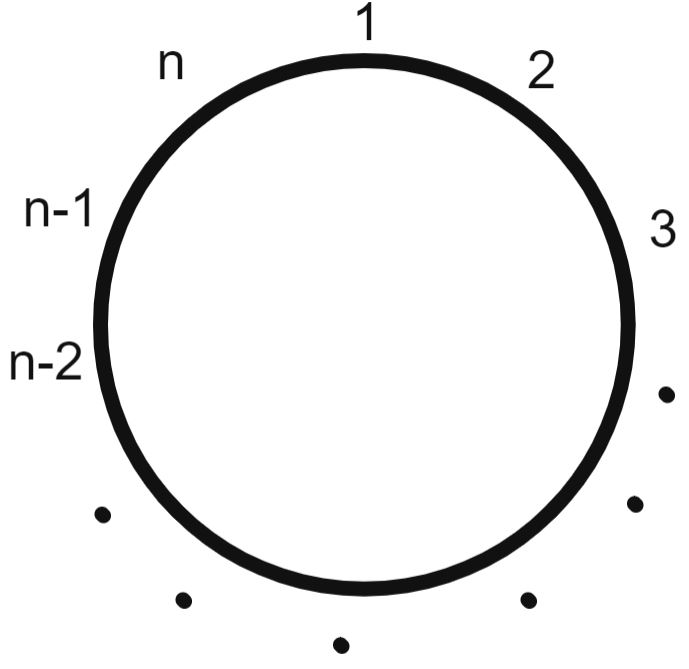
\includegraphics[width=\linewidth]{sol3} %тут поменять имя пикчи
    \end{figure}
    \end{minipage}
\end{minipage}

\textbf{Дефолтные математические знаки и символы:}\\
$\geqslant$,
$\leqslant$,
$a^{b}$,
$x_{i}$,
$\sqrt{a}$,
$\frac{a}{b}$,
$\displaystyle \frac{a}{b}$,
$\cdot$
$\;\Rightarrow\;$,
$\;\Leftrightarrow\;$,
$1{,}2$.
О промежутках:
$a\!b$,
$a\,b$,
$a\:b$,
$a\;b$,
$a\quad b$.

\textbf{Стандартные система и совокупность уравнений / неравенств:}\\
$\left\{
\begin{aligned}
f(x) &= 0 \\
g(x) &= 1
\end{aligned}\right.$

$\left[\begin{aligned}
&\left\{\begin{aligned}
f(x) &\geqslant a \\
g(x) &= b
\end{aligned}\right.\\
&\left\{\begin{aligned}
f(x) &< a \\
g(x) &= -b
\end{aligned}\right.
\end{aligned}\right.$

\subsection*{\textcolor{Emerald}{\textbf{Не математическое, но полезное:}}}
% комментарий в любом месте документа, который нигде не будет видно. Можно использовать для написания заметок-вопросов по задачам
\textbf{Пример таблицы:}

\begin{tabular}{|c|c|c|}
\hline
    $a$ & $b$ & текст
\\\hline
    $c$ & $d$ & мораль
\\\hline
\end{tabular}\\

\textbf{Отступы:} между\smallskip\\ строками\medskip\\ \textbf{Тире} --- это три дефиса.\\
\textbf{Списки:}
\begin{mylist}
\item [$\bullet$] это был пункт а
\item [2)] а это уже пункт номер 2 с изменённым заголовком
\end{mylist}

\subsection*{\textcolor{Emerald}{\textbf{Всё, неупомянутое выше (или если просто что-то не так):}}}
\begin{mylist}
\item [$\bullet$] Решение отдельных вопросов касательно ТеХа нужно искать в \href{https://www.mccme.ru/free-books/llang/newllang.pdf}{Львовском}.

\item [$\bullet$] Найти произвольный символ, который нужен, можно в \href{http://detexify.kirelabs.org/classify.html}{Detexify}.

\item [$\bullet$] Если возникли сомнения при решении, ответ практически ко всем задачам можно проверить с помощью \href{https://www.wolframalpha.com/}{WolframAlpha}.

\item [$\bullet$] Если в задаче нужно создать картинку, то лучше пока отложить эту задачу. Все графики планируется централизованно нарисовать (или перерисовать) в геогебре.

\item [\textcolor{brown}{\textbf{!!}}] Важно ставить \textcolor{red}{\textbf{$\spadesuit$}}
(или просто red) в тело задачи в случае серьёзных вопросов к решению и какой-то вопиющей лажи.

\item [\textcolor{brown}{\textbf{!!}}] Важно ставить \textcolor{olive}{\textbf{$\spadesuit$}}
(или просто olive) в тело задачи в случае не самого удачного текста и кривых отступов.
\end{mylist}

\subsection*{\textcolor{Violet}{\textbf{Комментарии:}}}% а также невидимые комментарии - так можно оставлять заметки-вопросы прямо в задаче, чтобы потом было понятно, в чём вопрос.
\begin{mylist}
\item [$\skull$] Переставлять задачи местами --- очень плохая идея.

\item [$\smiley$] При двойном клике по тексту pdf справа происходит автоматический переход к этому месту в латех-коде, а для обратного перехода можно нажать стрелку вправо (висит сверху между pdf и латех-кодом).

\item [$\smiley$] Если есть размышления, дописывать red/olive к задаче или не дописывать, то лучше всё-таки дописать.

\item [$\skull$] Самое плохое, что можно сделать --- написать в любое поле из трёх (НаписанноеРешение/ВерныйОтвет/Подсказка) только половину того, что надо, никак это не отметить, и потом пойти дальше.\\ Нужно в этот момент писать red/olive в случайном месте задачи, чтобы потом вычислить это с помощью Ctrl+F по всему документу (и это то, что потом будет делаться долго и тщательно)
\end{mylist}

\newpage
\setcounter{num}{1133}

\hypertarget{9.2}{{\centering\section*{\bigskip\\\textcolor{Blue}{\hyperlink{start2}{\textcolor{Blue}{9.2}} Неравенства с одной переменной.}\vspace{-5mm}}}}

\begin{problem}{Рациональные неравенства. Метод интервалов.}{9.2.1}{79I}{(лёгкая)}
{Решить неравенство: $\;\displaystyle x \geqslant \frac{9x + 15}{x + 11}$.}
{НаписанноеРешение}
{ВерныйОтвет}{Подсказка}
\end{problem}

\begin{problem}{Рациональные неравенства. Метод интервалов.}{9.2.1}{79I}{(лёгкая)}
{Решить двойное неравенство: $\;\displaystyle 0 < r < \frac{r + 6}{r + 4}$.}
{НаписанноеРешение}
{ВерныйОтвет}{Подсказка}
\end{problem}

\begin{problem}{Рациональные неравенства. Метод интервалов.}{9.2.1}{79I}{(лёгкая)}
{Решить неравенство: $\;\displaystyle -s - 6 > -\frac{39}{s - 4}$.}
{НаписанноеРешение}
{ВерныйОтвет}{Подсказка}
\end{problem}

\begin{problem}{Рациональные неравенства. Метод интервалов.}{9.2.1}{79I}{(лёгкая)}
{Решить неравенство: $\;\displaystyle (w + 1)(w - 2)(w + 3) > 0$.}
{НаписанноеРешение}
{ВерныйОтвет}{Подсказка}
\end{problem}

\begin{problem}{Рациональные неравенства. Метод интервалов.}{9.2.1}{79I}{(лёгкая)}
{Решить неравенство: $\displaystyle \;x(x - 4)(x - 5)(x + 1) \leqslant 0$.}
{НаписанноеРешение}
{ВерныйОтвет}{Подсказка}
\end{problem}

\begin{problem}{Рациональные неравенства. Метод интервалов.}{9.2.1}{79I}{(лёгкая)}
{Решить неравенство: $\displaystyle \;(y - 2)^{2} \leqslant 0$.}
{НаписанноеРешение}
{ВерныйОтвет}{Подсказка}
\end{problem}

\begin{problem}{Рациональные неравенства. Метод интервалов.}{9.2.1}{79I}{(лёгкая)}
{Решить неравенство: $\displaystyle\; z^{2}(z - 1)^{2}(z + 2)(z - 4)(z + 5)^{3} \geqslant 0$.}
{НаписанноеРешение}
{ВерныйОтвет}{Подсказка}
\end{problem}

\begin{problem}{Рациональные неравенства. Метод интервалов.}{9.2.1}{79I}{(лёгкая)}
{Найти все целые решения неравенства $\;\displaystyle \frac{x^{2} + x - 6}{x^{2} + 4x + 4} \leqslant 0$.}
{НаписанноеРешение}
{ВерныйОтвет}{Подсказка}
\end{problem}

\begin{problem}{Рациональные неравенства. Метод интервалов.}{9.2.1}{79I}{(лёгкая)}
{Решить неравенство: $\displaystyle \;(2x - x^{2})(2x + 6) > 0$.}
{НаписанноеРешение}
{ВерныйОтвет}{Подсказка}
\end{problem}

\begin{problem}{Рациональные неравенства. Метод интервалов.}{9.2.1}{79I}{(лёгкая)}
{Решить неравенство: $\displaystyle \;(-s^{2} - 2)(s^{3} - 4s^{2}) \geqslant 0$.}
{НаписанноеРешение}
{ВерныйОтвет}{Подсказка}
\end{problem}

\begin{problem}{Рациональные неравенства. Метод интервалов.}{9.2.1}{79I}{(лёгкая)}
{Решить неравенство: $\displaystyle \;p^{3} \geqslant 169p$.}
{НаписанноеРешение}
{ВерныйОтвет}{Подсказка}
\end{problem}

\begin{problem}{Рациональные неравенства. Метод интервалов.}{9.2.1}{79I}{(лёгкая)}
{Решить неравенство: $\displaystyle \;(3 + 5\alpha - 2\alpha^{2})(-\alpha - \alpha^{2})(2\alpha^{2} - \alpha) > 0$.}
{НаписанноеРешение}
{ВерныйОтвет}{Подсказка}
\end{problem}

\begin{problem}{Рациональные неравенства. Метод интервалов.}{9.2.1}{79I}{(лёгкая)}
{Решить неравенство: $\displaystyle \;(t^{2} - 25)(t^{2} - 6t + 5) \leqslant 0$.}
{НаписанноеРешение}
{ВерныйОтвет}{Подсказка}
\end{problem}

\begin{problem}{Рациональные неравенства. Метод интервалов.}{9.2.1}{79I}{(лёгкая)}
{Решить неравенство: $\displaystyle \;\frac{4 - x}{4 - 2x} \geqslant \frac{7x + 2}{2x - 4}$.}
{НаписанноеРешение}
{ВерныйОтвет}{Подсказка}
\end{problem}

\begin{problem}{Рациональные неравенства. Метод интервалов.}{9.2.1}{79I}{(лёгкая)}
{Решить неравенство: $\displaystyle \;(q^{4} - 9q^{2})(1 - q)(-q^{2} - 3) > 0$.}
{НаписанноеРешение}
{ВерныйОтвет}{Подсказка}
\end{problem}

\begin{problem}{Рациональные неравенства. Метод интервалов.}{9.2.1}{79I}{(лёгкая)}
{Решить неравенство: $\displaystyle \;\frac{8 - y^{2}}{y + 2} \geqslant 1$.}
{НаписанноеРешение}
{ВерныйОтвет}{Подсказка}
\end{problem}

\begin{problem}{Рациональные неравенства. Метод интервалов.}{9.2.1}{79I}{(лёгкая)}
{Решить неравенство: $\displaystyle \;\frac{3\beta^{3} - \beta^{4} + 4\beta^{2}}{\beta^{2} + \beta + 2} > 0$.}
{НаписанноеРешение}
{ВерныйОтвет}{Подсказка}
\end{problem}

\begin{problem}{Рациональные неравенства. Метод интервалов.}{9.2.1}{79I}{(лёгкая)}
{Решить неравенство: $\displaystyle \;\frac{z^{2}}{z^{2} + 1} \leqslant 0$.}
{НаписанноеРешение}
{ВерныйОтвет}{Подсказка}
\end{problem}

\begin{problem}{Рациональные неравенства. Метод интервалов.}{9.2.1}{79I}{(лёгкая)}
{Найти натуральные числа $n$, для которых верно неравенство: $\displaystyle \;\frac{5n + 1}{n - 1} \geqslant 2n + 2$.}
{НаписанноеРешение}
{ВерныйОтвет}{Подсказка}
\end{problem}

\begin{problem}{Рациональные неравенства. Метод интервалов.}{9.2.1}{79I}{*}
{Решить неравенство: $\displaystyle \;x^{3} - 2x^{2} - 5x + 6 < 0$.}
{НаписанноеРешение}
{ВерныйОтвет}{Подсказка}
\end{problem}

\begin{problem}{Рациональные неравенства. Метод интервалов.}{9.2.1}{79I}{(лёгкая)}
{Решить неравенство: $\displaystyle \;x > \frac{-8x - 20}{x - 17}$.}
{НаписанноеРешение}
{ВерныйОтвет}{Подсказка}
\end{problem}

\begin{problem}{Рациональные неравенства. Метод интервалов.}{9.2.1}{79I}{(лёгкая)}
{Решить неравенство: $\displaystyle \;x \leqslant \frac{2x + 18}{x - 1}$.}
{НаписанноеРешение}
{ВерныйОтвет}{Подсказка}
\end{problem}

\begin{problem}{Рациональные неравенства. Метод интервалов.}{9.2.1}{79I}{(лёгкая)}
{Решить неравенство: $\;(-x^{2} - 2)(x^{4} - 4x^{2}) \geqslant 0$.}
{НаписанноеРешение}
{ВерныйОтвет}{Подсказка}
\end{problem}

\begin{problem}{Рациональные неравенства. Метод интервалов.}{9.2.1}{79I}{(лёгкая)}
{Решить неравенство: $\displaystyle\;\frac{(4x - 4)(1 + x)(5 - x)}{(x + 2)^{2} - x - 22} < 0$.}
{НаписанноеРешение}
{ВерныйОтвет}{Подсказка}
\end{problem}

\begin{problem}{Рациональные неравенства. Метод интервалов.}{9.2.1}{79I}{(лёгкая)}
{Решить неравенство: $\;x^{2} - 5x^{3} - 66x > 0$.}
{НаписанноеРешение}
{ВерныйОтвет}{Подсказка}
\end{problem}

\begin{problem}{Рациональные неравенства. Метод интервалов.}{9.2.1}{79I}{(лёгкая)}
{Решить неравенство: $\;x^{3} - 9x < 4x^{2} - 36$.}
{НаписанноеРешение}
{ВерныйОтвет}{Подсказка}
\end{problem}

\begin{problem}{Рациональные неравенства. Метод интервалов.}{9.2.1}{79I}{(лёгкая)}
{Решить неравенство: $\;(3x - 6)(x - x^{2}) > 0$.}
{НаписанноеРешение}
{ВерныйОтвет}{Подсказка}
\end{problem}

\begin{problem}{Рациональные неравенства. Метод интервалов.}{9.2.1}{79I}{(лёгкая)}
{Решить неравенство: $\;(x^{2} - 4)(x^{2} - 3x + 2) < 0$.}
{НаписанноеРешение}
{ВерныйОтвет}{Подсказка}
\end{problem}

\begin{problem}{Рациональные неравенства. Метод интервалов.}{9.2.1}{79I}{(лёгкая)}
{Решить неравенство: $\displaystyle\;\frac{3x^{3} - x^{4} + 4x^{2}}{x^{2} + x + 2} > 0$.}
{НаписанноеРешение}
{ВерныйОтвет}{Подсказка}
\end{problem}

\begin{problem}{Рациональные неравенства. Метод интервалов.}{9.2.1}{9I}{(лёгкая)}
{Решить неравенство: $\;(2x - 4)^{2}(2x - 7) \geqslant 0$.}
{НаписанноеРешение}
{ВерныйОтвет}{Подсказка}
\end{problem}

\begin{problem}{Рациональные неравенства. Метод интервалов.}{9.2.1}{9I}{(лёгкая)}
{Найти наибольшее целое решение неравенства: $\:(2x - 8)(4 + x)^{2}(1 - x)(1 + x)^{6} > 0$.

}
{НаписанноеРешение}
{ВерныйОтвет}{Подсказка}
\end{problem}

\begin{problem}{Рациональные неравенства. Метод интервалов.}{9.2.1}{9I}{(лёгкая)}
{Решить неравенство: $\;(4x - 4)(1 + x)(5 - x)^{3} > 0$.}
{НаписанноеРешение}
{ВерныйОтвет}{Подсказка}
\end{problem}

\begin{problem}{Рациональные неравенства. Метод интервалов.}{9.2.1}{9D}{(лёгкая)}
{Решить неравенство: $\displaystyle \:x + \frac{1}{x} \leqslant \frac{5}{2}$.}
{НаписанноеРешение}
{ВерныйОтвет}{Подсказка}
\end{problem}

\begin{problem}{Рациональные неравенства. Метод интервалов.}{9.2.1}{9D}{(лёгкая)}
{Решить неравенство: $\displaystyle \;\frac{x^{2} - 14x + 48}{x + 6} \geqslant 0$.}
{НаписанноеРешение}
{ВерныйОтвет}{Подсказка}
\end{problem}

\begin{problem}{Рациональные неравенства. Метод интервалов.}{9.2.1}{9D}{(лёгкая)}
{Решить неравенство: $\displaystyle \;\frac{-2x}{x^{3} - 4x^{2} - 21x} \leqslant 0$.}
{НаписанноеРешение}
{ВерныйОтвет}{Подсказка}
\end{problem}

\begin{problem}{Рациональные неравенства. Метод интервалов.}{9.2.1}{9D}{(лёгкая)}
{Решить неравенство: $\displaystyle \;\frac{(5x^{2} - 5x - 150) \cdot (x^{2} + 7x - 8)}{-x^{3} + 9x^{2} - 20x} > 0$.}
{НаписанноеРешение}
{ВерныйОтвет}{Подсказка}
\end{problem}

\begin{problem}{Рациональные неравенства. Метод интервалов.}{9.2.1}{9D}{(лёгкая)}
{Решить неравенство: $\displaystyle\; \frac{3}{x - 3} > \frac{2}{x + 2} - 3$.}
{НаписанноеРешение}
{ВерныйОтвет}{Подсказка}
\end{problem}

\begin{problem}{Рациональные неравенства. Метод интервалов.}{9.2.1}{9D}{(лёгкая)}
{Решить неравенство: $\;\displaystyle \frac{5}{x + 4} - 3 \leqslant \frac{6}{x - 2}$.}
{НаписанноеРешение}
{ВерныйОтвет}{Подсказка}
\end{problem}

\begin{problem}{Рациональные неравенства. Метод интервалов.}{9.2.1}{9D}{(лёгкая)}
{Решить неравенство: $\;\displaystyle \frac{4}{x^{2} - 4} + 2 \leqslant \frac{1}{x - 2}$.}
{НаписанноеРешение}
{ВерныйОтвет}{Подсказка}
\end{problem}

\begin{problem}{Рациональные неравенства. Метод интервалов.}{9.2.1}{9D}{(лёгкая)}
{Решить неравенство: $\;\displaystyle \frac{x^{3} - 8}{x^{2} + 5x - 6} > 0$.}
{НаписанноеРешение}
{ВерныйОтвет}{Подсказка}
\end{problem}

\begin{problem}{Рациональные неравенства. Метод интервалов.}{9.2.1}{9D}{(лёгкая)}
{Решить неравенство: $\displaystyle \;(x - 1)(x - 2)^{2}(x - 3)^{3}(x - 4)^{4} \leqslant 0$.}
{НаписанноеРешение}
{ВерныйОтвет}{Подсказка}
\end{problem}

\begin{problem}{Рациональные неравенства. Метод интервалов.}{9.2.1}{9D}{(лёгкая)}
{Решить неравенство: $\displaystyle \;\frac{10 + 3x - x^{2}}{x^{2} - 3x + 2} \leqslant 1$.}
{НаписанноеРешение}
{ВерныйОтвет}{Подсказка}
\end{problem}

\begin{problem}{Рациональные неравенства. Метод интервалов.}{9.2.1}{9D}{(лёгкая)}
{Решить неравенство: $\displaystyle\; \frac{1}{x + 6} + \frac{1}{x - 2} \geqslant \frac{1}{x - 3}$.}
{НаписанноеРешение}
{ВерныйОтвет}{Подсказка}
\end{problem}

\begin{problem}{Рациональные неравенства. Метод интервалов.}{9.2.1}{9D}{(лёгкая)}
{Решить неравенство: $\displaystyle\; \frac{1}{2x^{2} + 3x} \leqslant \frac{1}{3x - 2x^{3}}$.}
{НаписанноеРешение}
{ВерныйОтвет}{Подсказка}
\end{problem}

\begin{problem}{Рациональные неравенства. Метод интервалов.}{9.2.1}{9D}{(лёгкая)}
{Решить неравенство: $\displaystyle\; 1 + \frac{16}{x - 3} \leqslant \frac{5x + 1}{(x + 2)(x - 3)}$.}
{НаписанноеРешение}
{ВерныйОтвет}{Подсказка}
\end{problem}

\begin{problem}{Рациональные неравенства. Метод интервалов.}{9.2.1}{9D}{(лёгкая)}
{Решить неравенство: $\displaystyle\; \frac{(12 - x - x^{2})(3x - x^{2})}{(9 - 4x^{2})(1 - x^{2})^{6}} > 0$.}
{НаписанноеРешение}
{ВерныйОтвет}{Подсказка}
\end{problem}

\begin{problem}{Рациональные неравенства. Метод интервалов.}{9.2.1}{9D}{(лёгкая)}
{Решить неравенство: $\displaystyle\; -x \geqslant \frac{8x - 28}{x - 11}$.}
{НаписанноеРешение}
{ВерныйОтвет}{Подсказка}
\end{problem}

\begin{problem}{Рациональные неравенства. Метод интервалов.}{9.2.1}{9D}{(лёгкая)}
{Решить неравенство: $\displaystyle\; \frac{2}{x - 5} + 1 \geqslant \frac{2}{x + 1}$.}
{НаписанноеРешение}
{ВерныйОтвет}{Подсказка}
\end{problem}

\begin{problem}{Рациональные неравенства. Метод интервалов.}{9.2.1}{9D}{(лёгкая)}
{Решить неравенство: $\displaystyle\; \frac{5}{2x - 2} \leqslant \frac{7}{3x + 3} + \frac{1}{6}$.}
{НаписанноеРешение}
{ВерныйОтвет}{Подсказка}
\end{problem}

\begin{problem}{Рациональные неравенства. Метод интервалов.}{9.2.1}{9D}{(лёгкая)}
{Решить неравенство: $\displaystyle\; \frac{x}{x + 3} + \frac{x - 5}{x} < \frac{2x}{3 - x}$.}
{НаписанноеРешение}
{ВерныйОтвет}{Подсказка}
\end{problem}

\begin{problem}{Рациональные неравенства. Метод интервалов.}{9.2.1}{9D}{(лёгкая)}
{Решить неравенство: $\displaystyle\; \frac{2}{x + 3} + 1 \leqslant \frac{6}{5 - x}$.}
{НаписанноеРешение}
{ВерныйОтвет}{Подсказка}
\end{problem}

\begin{problem}{Рациональные неравенства. Метод интервалов.}{9.2.1}{X}{(лёгкая)}
{Найти решение неравенства $\displaystyle \; \frac{(x - 1)(x + 1)}{(x - 1)^{2}} > 2$.}
{НаписанноеРешение}
{ВерныйОтвет}{Подсказка}
\end{problem}

\begin{problem}{Системы неравенств.}{9.2.3}{9I}{(лёгкая)}
{Решить систему неравенств $\;\left\{
\begin{aligned}
    \: t^{2} - 6t + 5 &\leqslant 0\\
    \: \frac{4\sqrt{3} - 7}{t^{2} - 8t + 15} &\leqslant 0
\end{aligned}\right.$}
{НаписанноеРешение}
{ВерныйОтвет}{Подсказка}
\end{problem}

\begin{problem}{Системы неравенств.}{9.2.3}{9I}{(лёгкая)}
{a) Решить систему неравенств:
$\;\displaystyle \left\{\begin{aligned}
    t^{2} - 6t\quad\;\; & \leqslant 0\\
    \frac{3\sqrt{7} - 8}{4t^{2} - 28t + 40} & \leqslant 0
\end{aligned}\right.$\smallskip\\
b) Найти сумму всех целочисленных решений данного неравенства.}
{НаписанноеРешение}
{ВерныйОтвет}{Подсказка}
\end{problem}

\begin{problem}{Системы неравенств.}{9.2.3}{9D}{(лёгкая)}
{Решить систему неравенств: $\;\left\{\begin{aligned}
    \frac{5x + 1}{x + 3} &\geqslant 0\\
    4x - 3 &\leqslant 0
\end{aligned}\right.$}
{НаписанноеРешение}
{ВерныйОтвет}{Подсказка}
\end{problem}

\begin{problem}{Системы неравенств.}{9.2.3}{X}{(лёгкая)}
{Изобразить на прямой решение системы неравенств: $\;\left\{\begin{aligned}
    -5 + 3x &\leqslant -2x\\
    6x + 11 &> 2 + x
\end{aligned}\right.$}
{НаписанноеРешение}
{ВерныйОтвет}{Подсказка}
\end{problem}

\begin{problem}{Неравенства с модулем.}{9.2.5}{9I}{(лёгкая)}
{Решить неравенство с модулем: $\;|x^{2} - 6x + 8| \geqslant x - 2$.}
{НаписанноеРешение}
{ВерныйОтвет}{Подсказка}
\end{problem}

\begin{problem}{Неравенства с модулем.}{9.2.5}{9I}{(лёгкая)}
{Решить неравенство: $\displaystyle \,\left|x + \frac{1}{x}\right| \leqslant 3$.}
{НаписанноеРешение}
{ВерныйОтвет}{Подсказка}
\end{problem}

\begin{problem}{Неравенства с модулем.}{9.2.5}{9D}{(лёгкая)}
{Решить неравенство: $\displaystyle\; |x^{2} + 2x - 63| \geqslant 64 - 4x$.}
{НаписанноеРешение}
{ВерныйОтвет}{Подсказка}
\end{problem}

\begin{problem}{Неравенства с модулем.}{9.2.5}{9D}{(лёгкая)}
{Решить неравенство: $\displaystyle\; |x^{2} - 5| < x + 1$.}
{НаписанноеРешение}
{ВерныйОтвет}{Подсказка}
\end{problem}

\begin{problem}{Неравенства с модулем.}{9.2.5}{9D}{(лёгкая)}
{Решить неравенство: $\; |x^{2} + 10x + 9| \leqslant \frac{1}{4} \cdot (x^{2} - 6x + 21)$.}
{НаписанноеРешение}
{ВерныйОтвет}{Подсказка}
\end{problem}

\begin{problem}{Неравенства с модулем.}{9.2.5}{9D}{(лёгкая)}
{Решить неравенство: $\displaystyle \;x^{2} - 7 \geqslant |3x - 7|$.}
{НаписанноеРешение}
{ВерныйОтвет}{Подсказка}
\end{problem}

\begin{problem}{Неравенства с модулем.}{9.2.5}{9D}{*}
{Решить неравенство: $\displaystyle \;\frac{|x - 2| - |x + 7|}{2 - |x + 3|} \leqslant -1$.}
{НаписанноеРешение}
{ВерныйОтвет}{Подсказка}
\end{problem}

\begin{problem}{Неравенства с модулем.}{9.2.5}{9D}{*}
{Решить неравенство: $\displaystyle \;\frac{x + 1}{2|x - 1| - |x + 2|} \geqslant 1$.}
{НаписанноеРешение}
{ВерныйОтвет}{Подсказка}
\end{problem}

\begin{problem}{Неравенства с модулем.}{9.2.5}{9D}{(лёгкая)}
{Решить неравенство: $\;4x^{2} + 4x - \frac{1}{2} > |4x + 3{,}5|$.}
{НаписанноеРешение}
{ВерныйОтвет}{Подсказка}
\end{problem}

\begin{problem}{Неравенства с модулем.}{9.2.5}{9D red check roots}{(лёгкая)}
{Решить неравенство: $\displaystyle \;-|(x - 2)(x - 5)| \leqslant 1{,}9x - 7{,}7$.}
{НаписанноеРешение}
{ВерныйОтвет}{Подсказка}
\end{problem}

\begin{problem}{Неравенства с модулем.}{9.2.5}{9D}{(лёгкая)}
{Решить неравенство: $\;x^{2} + 4x + 7 < |8x + 4|$.}
{НаписанноеРешение}
{ВерныйОтвет}{Подсказка}
\end{problem}

\begin{problem}{Иррациональные неравенства.}{9.2.6}{79I}{(лёгкая)}
{Решить неравенство: $\displaystyle \,\sqrt{-36 - 13x} \geqslant -x$.}
{НаписанноеРешение}
{ВерныйОтвет}{Подсказка}
\end{problem}

\begin{problem}{Иррациональные неравенства.}{9.2.6}{79I}{(лёгкая)}
{Решить неравенство: $\displaystyle \,\sqrt{21 - 4x} > -x$.}
{НаписанноеРешение}
{ВерныйОтвет}{Подсказка}
\end{problem}

\begin{problem}{Иррациональные неравенства.}{9.2.6}{79I}{(лёгкая)}
{Решить неравенство: $\displaystyle \,\sqrt{12 + x} \leqslant x$.}
{НаписанноеРешение}
{ВерныйОтвет}{Подсказка}
\end{problem}

\begin{problem}{Иррациональные неравенства.}{9.2.6}{79I}{(лёгкая)}
{Решить неравенство: $\displaystyle \,\sqrt{-35 + 12x} < x$.}
{НаписанноеРешение}
{ВерныйОтвет}{Подсказка}
\end{problem}

\begin{problem}{Иррациональные неравенства.}{9.2.6}{79I}{(лёгкая)}
{Решить неравенство: $\displaystyle \,\sqrt{-x - 4} < -x - 4$.}
{НаписанноеРешение}
{ВерныйОтвет}{Подсказка}
\end{problem}

\begin{problem}{Иррациональные неравенства.}{9.2.6}{79I}{(лёгкая)}
{Решить неравенство: $\displaystyle \,\sqrt{-9x - 32} \geqslant x + 2$.}
{НаписанноеРешение}
{ВерныйОтвет}{Подсказка}
\end{problem}

\begin{problem}{Иррациональные неравенства.}{9.2.6}{79I}{(лёгкая)}
{Решить неравенство $\displaystyle \sqrt{-x - 3} > -x - 3$ графически, нарисовав графики обеих функций.}
{НаписанноеРешение}
{ВерныйОтвет}{Подсказка}
\end{problem}

\begin{problem}{Иррациональные неравенства.}{9.2.6}{79I}{(лёгкая)}
{Решить неравенство $\displaystyle \sqrt{56 + x} \geqslant -x$ графически, нарисовав графики обеих\\ функций.}
{НаписанноеРешение}
{ВерныйОтвет}{Подсказка}
\end{problem}

\begin{problem}{Иррациональные неравенства.}{9.2.6}{79I}{(лёгкая)}
{Решить неравенство $\displaystyle x + 3 < \sqrt{6x + 90}$ аналитически.}
{НаписанноеРешение}
{ВерныйОтвет}{Подсказка}
\end{problem}

\begin{problem}{Иррациональные неравенства.}{9.2.6}{79I}{(лёгкая)}
{Решить неравенство: $\displaystyle \,\sqrt{18 + 7x} > x$.}
{НаписанноеРешение}
{ВерныйОтвет}{Подсказка}
\end{problem}

\begin{problem}{Иррациональные неравенства.}{9.2.6}{79I}{(лёгкая)}
{Решить неравенство: $\displaystyle\, \sqrt{4x^{2} + 8x - 140} > -1$.}
{НаписанноеРешение}
{ВерныйОтвет}{Подсказка}
\end{problem}

\begin{problem}{Иррациональные неравенства.}{9.2.6}{79I}{(лёгкая)}
{Решить неравенство: $\displaystyle\, \sqrt{2x^{2} + 6x - 8} \leqslant x + 4$.}
{НаписанноеРешение}
{ВерныйОтвет}{Подсказка}
\end{problem}

\begin{problem}{Иррациональные неравенства.}{9.2.6}{9I}{(лёгкая)}
{Указать наибольшее решение неравенства $\,2\sqrt{16 - x^{2}} < x + 8$.}
{НаписанноеРешение}
{ВерныйОтвет}{Подсказка}
\end{problem}

\begin{problem}{Иррациональные неравенства.}{9.2.6}{X}{(лёгкая)}
{Решить иррациональное неравенство: $\, \frac{1}{3} \cdot (x + 2) > \sqrt{x}$. Найти ОДЗ.}
{НаписанноеРешение}
{ВерныйОтвет}{Подсказка}
\end{problem}

\begin{problem}{Задачи с параметром, сводящиеся к решению неравенств.}{9.2.7}{9D}{(лёгкая)}
{Найти значения $a$, при которых неравенство $\displaystyle \left(a + 2\right)x^{2} + (2a + 3)x + a + 6 \leqslant 0$ выполнено для всех действительных $x$.}
{НаписанноеРешение}
{ВерныйОтвет}{Подсказка}
\end{problem}

\begin{problem}{Задачи с параметром, сводящиеся к решению неравенств.}{9.2.7}{9D}{(лёгкая)}
{Найти значения $a$, при которых неравенство $\displaystyle \left(a - 1\right)x^{2} - (7 + 3a)x - 2a + 5 < 0$ выполнено для всех действительных $x$.}
{НаписанноеРешение}
{ВерныйОтвет}{Подсказка}
\end{problem}

\begin{problem}{Задачи с параметром, сводящиеся к решению неравенств.}{9.2.7}{9D}{(лёгкая)}
{Установить, при каких значениях параметра $a$ решением неравенства $\displaystyle \frac{a}{x - 3} + 1 \leqslant \frac{a}{x + 3}$ будет только один промежуток.}
{НаписанноеРешение}
{ВерныйОтвет}{Подсказка}
\end{problem}

\begin{problem}{Задачи с параметром, сводящиеся к решению неравенств.}{9.2.7}{9D}{(лёгкая)}
{Решить биквадратное уравнение с параметром, рассмотрев все случаи: $$3x^{4} + (3a + 1)x^{2} + a = 0.$$

}
{НаписанноеРешение}
{ВерныйОтвет}{Подсказка}
\end{problem}

\begin{problem}{Задачи с параметром, сводящиеся к решению неравенств.}{9.2.7}{9D}{(лёгкая)}
{Решить уравнение $\displaystyle 6t^{4} + (2 - 3a - 2a^{2})t^{2} + a^{3} - a = 0$, указав как число корней уравнения зависит от параметра $a$.}
{НаписанноеРешение}
{ВерныйОтвет}{Подсказка}
\end{problem}

\begin{problem}{Задачи с параметром, сводящиеся к решению неравенств.}{9.2.7}{9D}{(лёгкая)}
{Найти все значения параметра $a$, при которых уравнение $x^{4} - (a + 1)x^{2} - 20a^{2} + 41a - 20 = 0$ имеет 4 корня.}
{НаписанноеРешение}
{ВерныйОтвет}{Подсказка}
\end{problem}

\begin{problem}{Задачи с параметром, сводящиеся к решению неравенств.}{9.2.7}{9D}{(лёгкая)}
{Найти все значения параметра $a$, при которых уравнение $x^{4} - (2a + 4)x^{2} - 3a^{2} + 8a + 3 = 0$ имеет 4 корня.}
{НаписанноеРешение}
{ВерныйОтвет}{Подсказка}
\end{problem}

\begin{problem}{Задачи с параметром, сводящиеся к решению неравенств.}{9.2.7}{9D}{(лёгкая)}
{Найти все значения параметра $a$, при которых биквадратное уравнение \\$x^{4} + (3a - 7)x^{2} - 18a + 6 = 0$ имеет 4 корня.}
{НаписанноеРешение}
{ВерныйОтвет}{Подсказка}
\end{problem}

\begin{problem}{Задачи с параметром, сводящиеся к решению неравенств.}{9.2.7}{9D}{(лёгкая)}
{Найти все значения параметра $a$, при которых неравенство $(a - 3)x^{2} - (a + 1)x + a + 1 \geqslant 0$ выполняется при всех действительных $x$.}
{НаписанноеРешение}
{ВерныйОтвет}{Подсказка}
\end{problem}

\begin{problem}{Задачи с параметром, сводящиеся к решению неравенств.}{9.2.7}{9D}{(лёгкая)}
{Найти все значения параметра $a$, при которых уравнение $x^{4} - (2a + 3)x^{2} + 6a = 0$ имеет 4 корня.}
{НаписанноеРешение}
{ВерныйОтвет}{Подсказка}
\end{problem}

\begin{problem}{Задачи с параметром, сводящиеся к решению неравенств.}{9.2.7}{9D}{(лёгкая)}
{Найти положительные значения параметра $a$, при которых график функции \\$y = |x^{2} - 8x - a^{2} - a + 18|$ имеет ровно три общих точки с прямой $y = 4$.}
{НаписанноеРешение}
{ВерныйОтвет}{Подсказка}
\end{problem}

\begin{problem}{Задачи с параметром, сводящиеся к решению неравенств.}{9.2.7}{9D}{(лёгкая)}
{Найти все значения параметра $a$, при которых неравенство\\ $(a - 14)t^{2} + (2a + 8)t + a + 1 > 0$ выполняется при всех вещественных $t$.}
{НаписанноеРешение}
{ВерныйОтвет}{Подсказка}
\end{problem}

\begin{problem}{Задачи с параметром, сводящиеся к решению неравенств.}{9.2.7}{9D}{(лёгкая)}
{Найти все значения параметра $a$, при которых уравнение $y^{4} - (a + 7)y^{2} + 4a + 12 = 0$ имеет ровно три корня.}
{НаписанноеРешение}
{ВерныйОтвет}{Подсказка}
\end{problem}

\begin{problem}{Задачи с параметром, сводящиеся к решению неравенств.}{9.2.7}{9D}{(лёгкая)}
{Найти все значения параметра $c$, при которых неравенство $\displaystyle (c + 1)x^{2} + (c - 2)x + c - 2 \geqslant 0$ выполнено для всех действительных $x$.}
{НаписанноеРешение}
{ВерныйОтвет}{Подсказка}
\end{problem}

\begin{problem}{Задачи с параметром, сводящиеся к решению неравенств.}{9.2.7}{9D}{(лёгкая)}
{Найти все значения параметра $c$, при которых неравенство $x^{2} + (2c - 8)x + 4c + 5 \geqslant 0$ выполняется при всех вещественных $x$.}
{Данное выражение является квадратным трёхчленом при любом значении $c$. Поэтому нужно только выяснить, при каком значении параметра данная парабола принимает только неотрицательные значения. Для этого требуется выполнение только двух условий: во-первых, старший коэффициент должен быть больше 0, так как в противном случае ветви параболы пойдут вниз.\\ В нашем случае старший коэффициент от $c$ не зависит и равен $1 > 0$.\\ Во-вторых, данная парабола должна иметь не более 1 корня ($D \leqslant 0$). В нашем случае дискриминант зависит от $c$, запишем выражение: $D = (2c - 8)^2 - 4(4c + 5) \leqslant 0$ $\Rightarrow\; D = 4c^2 - 32c + 64 - 16c - 20 = 4c^2 - 48c + 44 \leqslant 0 \Rightarrow c^2 - 12c + 11 \leqslant 0$.\\
Решим соответствующее квадратное уравнение: теорема Виета даёт разложение $c^2 - 12c + 11 = (c - 1)(c - 11)$, и корнями уравнения являются $c = 1$ и $c = 11$.\\ Поэтому, решая квадратное неравенство на $c$, и учитывая, что парабола $c^2 - 12c + 11$ имеет положительный старший коэффициент, получаем ответ: $c \in [1; 11]$.\\ Границы входят в ответ, так как квадратное неравенство на $c$ нестрогое.}
{Неравенство выполняется $\forall x$ при $c \in [1; 11]$.}{Подсказка}
\end{problem}

\begin{problem}{Задачи с параметром, сводящиеся к решению неравенств.}{9.2.7}{9D}{(лёгкая)}
{Найти все значения параметра $a$, при которых биквадратное уравнение \\$x^{4} - 2(a + 2)x^{2} + a^{2} + 4a + 3 = 0$ имеет 4 корня.}
{НаписанноеРешение}
{ВерныйОтвет}{Подсказка}
\end{problem}

\begin{problem}{Задачи с параметром, сводящиеся к решению неравенств.}{9.2.7}{9D}{(лёгкая)}
{Определить значения параметра $a$, при которых уравнение $z^{2} + (a^{2} - a + 1)z - a^{3} - a = 0$ имеет единственное решение.}
{НаписанноеРешение}
{ВерныйОтвет}{Подсказка}
\end{problem}

\begin{problem}{Задачи с параметром, сводящиеся к решению неравенств.}{9.2.7}{9D}{(лёгкая)}
{Найти все значения параметра $c$, при которых неравенство $\displaystyle cx^{2} + (c + 1)x + 9c < 0$ выполняется при всех действительных $x$.}
{НаписанноеРешение}
{ВерныйОтвет}{Подсказка}
\end{problem}

\end{document}